\chapter{Getting Started}
\label{chap:starting}

\section{Hello Proofs}

The first step in using \why is to write a suitable input
file. When one wants to learn a programming language, one starts by
writing a basic program. Here is our first \why file, which is the file
\texttt{examples/hello\_proof.why} of the distribution. It contains a
small set of goals.
\lstinputlisting[language=why3]{../examples/hello_proof.why}

Any declaration must occur
inside a theory, which is in that example called HelloProof and
labeled with a comment inside double quotes. It contains three goals
named $G_1,G_2,G_3$. The first two are basic propositional goals,
whereas the third involves some integer arithmetic, and thus it
requires to import the theory of integer arithmetic from the \why
standard library, which is done by the \texttt{use} declaration above.

We don't give more details here about the syntax and refer to
Chapter~\ref{chap:syntax} for detailed explanations. In the following,
we show how this file is handled in the \why GUI
(Section~\ref{sec:gui}) then in batch mode using the \texttt{why3}
executable (Section~\ref{sec:batch}).


\section{Getting Started with the GUI}
\label{sec:gui}

The graphical interface allows to browse into a file or a set of
files, and check the validity of goals with external provers, in a
friendly way. This section presents the basic use of this GUI. Please
refer to Section~\ref{sec:ideref} for a more complete description.

\begin{figure}[tbp]
%HEVEA\centering
  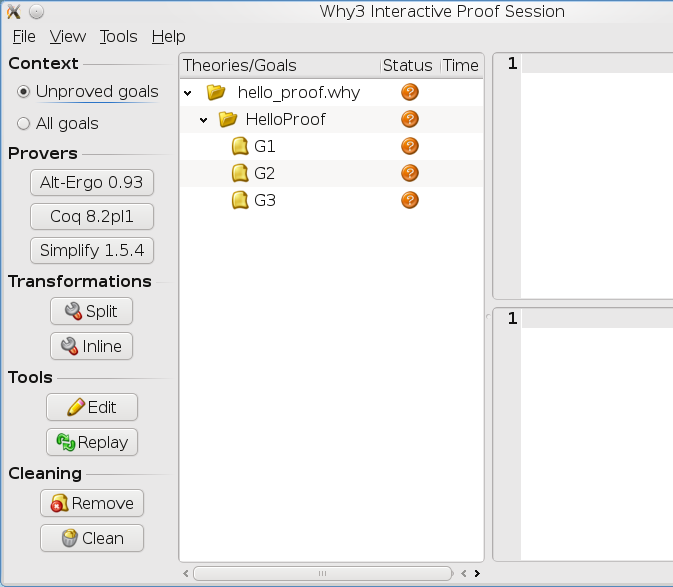
\includegraphics[width=\textwidth]{gui-0-70-1.png}
  \caption{The GUI when started the very first time}
  \label{fig:gui1}
\end{figure}

The GUI is launched on the file above as follows.
\begin{verbatim}
why3ide hello_proof.why
\end{verbatim}
When the GUI is started for the first time, you should get a window
which looks like the screenshot of Figure~\ref{fig:gui1}.

The left column is a tool bar which provides different actions to
apply on goals. The section ``Provers'' displays the provers that were
detected as installed on your computer\footnote{If not done yet, you
  must perform prover autodetection using \texttt{why3config
    --detect-provers}}. Three provers were detected, in this case
these are Alt-Ergo~\cite{ergo}, Coq~\cite{CoqArt} and
Simplify~\cite{simplify05}.

The middle part is a tree view that
allows to browse inside the theories.
% Initially, the item of this tree
% are closed. We can expand this view using the menu \textsf{View/Expand
%   all} or its shortcut \textsf{Ctrl-E}. This will result is something
% like the screenshot of Figure~\ref{fig:gui2}.
In this tree view, we have a structured view of the file: this file
contains one theory, itself containing three goals.


\begin{figure}[tbp]
%HEVEA\centering
 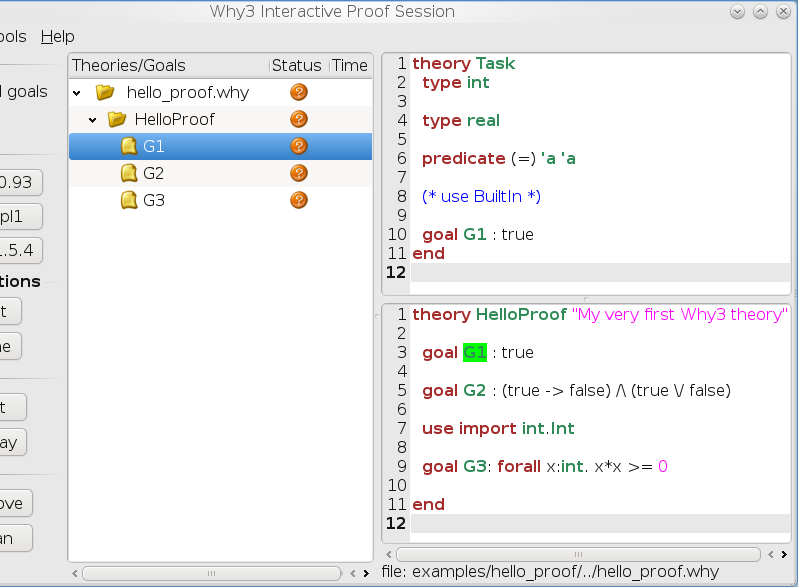
\includegraphics[width=\textwidth]{gui-0-70-2.png}
  \caption{The GUI with goal G1 selected}
  \label{fig:gui2}
\end{figure}
In Figure~\ref{fig:gui2}, we clicked on the row corresponding to
goal $G_1$. The \emph{task} associated with this goal is then
displayed on the top right, and the corresponding part of the input
file is shown on the bottom right part.


\subsection{Calling provers on goals}

You are now ready to call these provers on the goals. Whenever you
click on a prover button, this prover is called on the goal selected
in the tree view. You can select several goals at a time, either
by using multi-selection (typically by clicking while pressing the
\textsf{Shift} or \textsf{Ctrl} key) or by selecting the parent theory
or the parent file. Let us now select the theory ``HelloProof'' and
click on the \textsf{Simplify} button. After a short time, you should
get the display of Figure~\ref{fig:gui3}.

\begin{figure}[tbp]
%HEVEA\centering
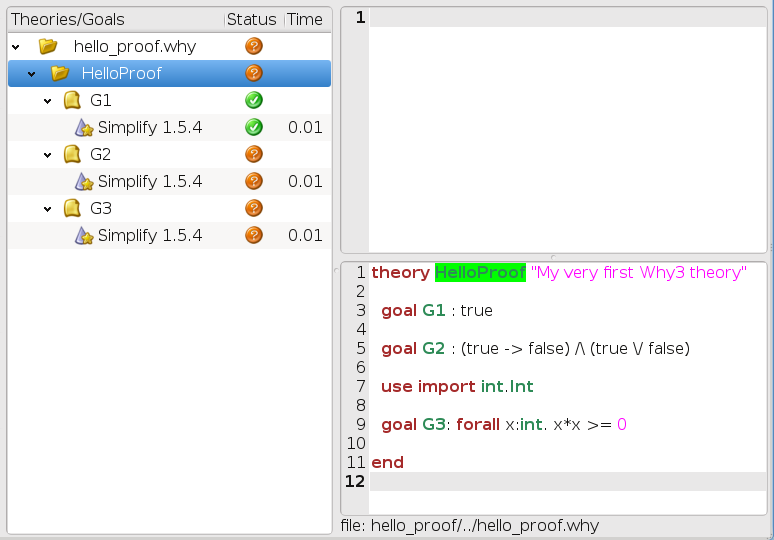
\includegraphics[width=\textwidth]{gui-0-70-3.png}
  \caption{The GUI after Simplify prover is run on each goal}
  \label{fig:gui3}
\end{figure}

The goal $G_1$ is now marked with a green ``checked'' icon in the
status column. This means that the goal is proved by the Simplify
prover. On the contrary, the two other goals are not proved, they remain
marked with an orange question mark.

You can immediately attempt to prove the remaining goals using another
prover, {\eg} Alt-Ergo, by clicking on the corresponding button. The
goal $G_3$ should be proved now, but not $G_2$.

\subsection{Applying transformations}

Instead of calling a prover on a goal, you can apply a transformation
to it.  Since $G_2$ is a conjunction, a possibility is to split it
into subgoals. You can do that by clicking on the \textsf{Split}
button of section ``Transformations'' of the left toolbar. Now you
have two subgoals, and you can try again a prover on them, for example
Simplify. We already have a lot of goals and proof attempts, so it is a good idea to close the sub-trees which are already proved: this can be done by the menu \textsf{View/Collapse proved goals}, or even better by its shortcut ``Ctrl-C''.
You should see now what is displayed on Figure~\ref{fig:gui4}.

\begin{figure}[tbp]
%HEVEA\centering
 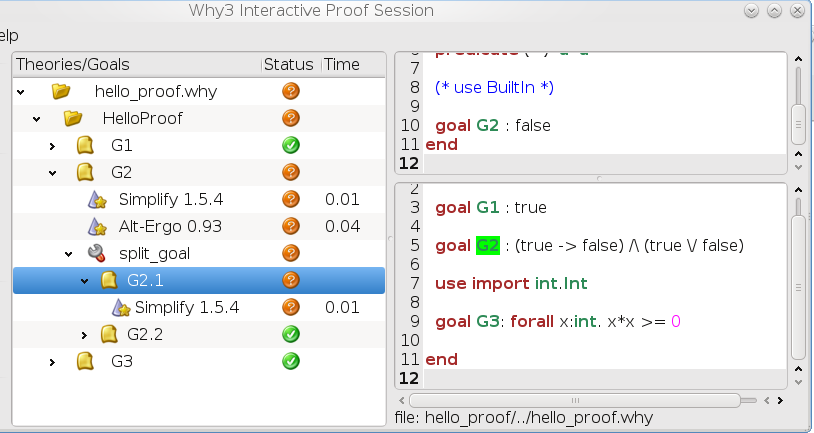
\includegraphics[width=\textwidth]{gui-0-70-4.png}
  \caption{The GUI after splitting goal $G_2$ and collapsing proved goals}
  \label{fig:gui4}
\end{figure}

The first part of goal $G_2$ is still unproved. As a last resort, we
can try to call the Coq proof assistant. The first step is to click on
the \textsf{Coq} button. A new sub-row appear for Coq, and
unsurprisingly the goal is not proved by Coq either. What can be done
now is editing the proof: select that row and then click on the
\textsf{Edit} button in section ``Tools'' of the toolbar. This should
launch the Coq proof editor, which is \texttt{coqide} by default (see
Section~\ref{sec:ideref} for details on how to configure this). You get
now a regular Coq file to fill in, as shown on Figure~\ref{fig:coqide}.
Please take care of the comments of this file. Only the part between
the two last comments can be modified. Moreover, these comments
themselves should not be modified at all, they are used to mark the
part you modify, in order to regenerate the file if the goal is
changed.

\begin{figure}[tbp]
%HEVEA\centering
  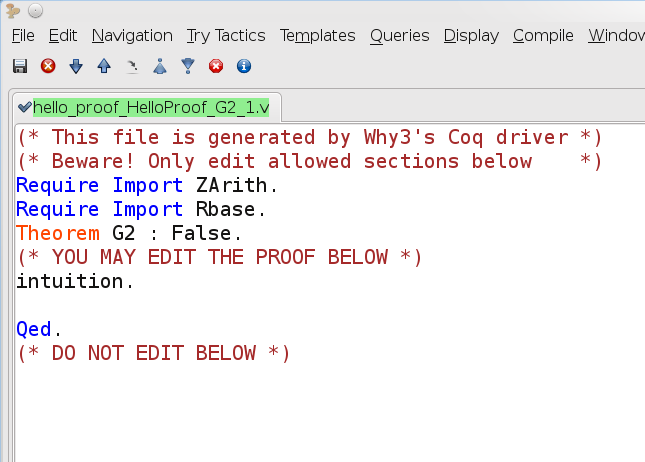
\includegraphics[width=\textwidth]{coqide-0-70.png}
  \caption{CoqIDE on subgoal 1 of $G_2$}
  \label{fig:coqide}
\end{figure}

Of course, in that particular case, the goal cannot be proved since it
is not valid. The only thing to do is to fix the input file, as
explained below.

\subsection{Modifying the input}

Currently, the GUI does not allow to modify the input file. You must
edit the file external by some editor of your choice. Let's assume we
change the goal $G_2$ by replacing the first occurrence of true by
false, \eg
\begin{whycode}
  goal G2 : (false -> false) /\ (true \/ false)
\end{whycode}
We can reload the modified file in the IDE using menu \textsf{File/Reload}, or the shortcut ``Ctrl-R''. We get the tree view shown on Figure~\ref{fig:gui5}.

\begin{figure}[tbp]
%HEVEA\centering
  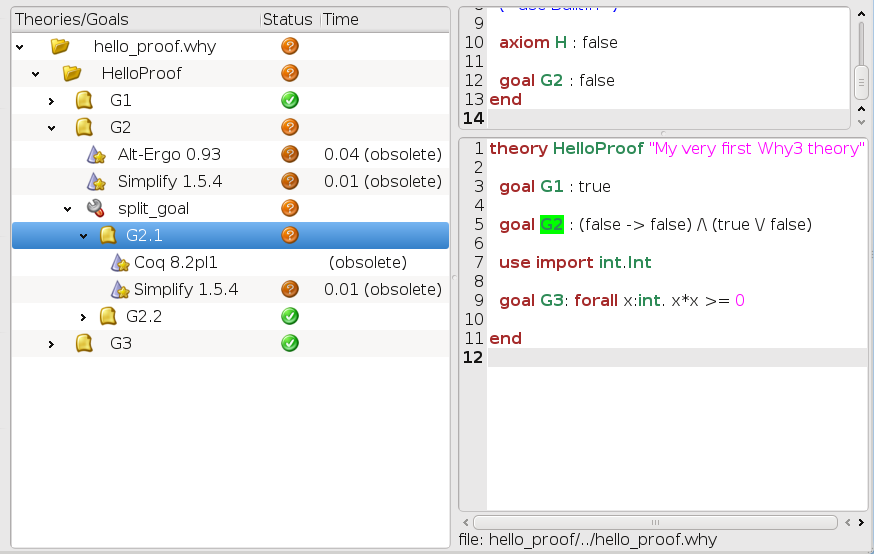
\includegraphics[width=\textwidth]{gui-0-70-5.png}
  \caption{File reloaded after modifying goal $G_2$}
  \label{fig:gui5}
\end{figure}

The important feature to notice first is that all the previous proof
attempts and transformations were saved in a database --- an XML file
created when the \why file was opened in the GUI for the first
time. Then, for all the goals that remain unchanged, the previous
proofs are shown again. For the parts that changed, the previous
proofs attempts are shown but marked with ``(obsolete)''\index{obsolete!proof attempt}
so that you
know the results are not accurate. You can now retry to prove all what
remains unproved using any of the provers.

\subsection{Replaying obsolete proofs}

Instead of pushing a prover's button to rerun its proofs, you can
\emph{replay} the existing but obsolete
proof attempts, by clicking on
the \textsf{Replay} button. By default, \textsf{Replay} only replays
proofs that were successful before. If you want to replay all of them,
you must select the context \textsf{all goals} at the top of the left
tool bar.

Notice that replaying can be done in batch mode, using the
\texttt{why3replayer} tool (see Section~\ref{sec:why3replayer}) For
example, running the replayer on the \texttt{hello\_proof} example is
as follows (assuming $G_2$ still is
\lstinline|(true -> false) /\ (true \/ false)|).
\begin{verbatim}
$ why3replayer hello_proof
Info: found directory 'hello_proof' for the project
Opening session...[Xml warning] prolog ignored
[Reload] file '../hello_proof.why'
[Reload] theory 'HelloProof'
[Reload] transformation split_goal for goal G2
 done
Progress: 9/9
 2/3
   +--file ../hello_proof.why: 2/3
      +--theory HelloProof: 2/3
         +--goal G2 not proved
Everything OK.
\end{verbatim}
The last line tells us that no difference was detected between the
current run and the informations in the XML file. The tree above
reminds us that the G2 is not proved.

\subsection{Cleaning}

You may want to clean some the proof attempts, \eg removing the
unsuccessful ones when a project is finally fully proved.

A proof or a transformation can be removed by selecting it and
clicking on button \textsf{Remove}. You must confirm the
removal. Beware that there is no way to undo such a removal.

The \textsf{Clean} button performs an automatic removal of all proofs
attempts that are unsuccessful, while there exists a successful proof
attempt for the same goal.

\section{Getting Started with the \why Command}
\label{sec:batch}

The why3 command allows to check the validity of goals with external
provers, in batch mode. This section presents the basic use of this
tool. Refer to Section~\ref{sec:why3ref} for a more complete
description of this tool and all its command-line options.

The very first time you want to use Why, you should proceed with
autodetection of external provers. We have already seen how to do
it in the \why GUI. On the command line, this is done as follows
(here ``\texttt{>}'' is the prompt):
\begin{verbatim}
> why3config --detect
\end{verbatim}
This prints some information messages on what detections are attempted. To know which
provers have been successfully detected, you can do as follows.
\begin{verbatim}
> why3 --list-provers
Known provers:
  alt-ergo (Alt-Ergo)
  coq (Coq)
  simplify (Simplify)
\end{verbatim}
The first word of each line is a unique identifier for the associated prover. We thus
have now the three provers Alt-Ergo~\cite{ergo}, Coq~\cite{CoqArt} and
Simplify~\cite{simplify05}.

Let's assume now we want to run Simplify on the HelloProof
example. The command to type and its output are as follows, where the
\verb|-P| option is followed by the unique prover identifier (as shown
by \texttt{--list-provers} option).
\begin{verbatim}
> why3 -P simplify hello_proof.why
hello_proof.why HelloProof G1 : Valid (0.10s)
hello_proof.why HelloProof G2 : Unknown: Unknown (0.01s)
hello_proof.why HelloProof G3 : Unknown: Unknown (0.00s)
\end{verbatim}
Unlike \why GUI, the command-line tool does not save the proof attempts
or applied transformations in a database.

We can also specify which goal or goals to prove. This is done by giving
first a theory identifier, then goal identifier(s). Here is the way to
call Alt-Ergo on goals $G_2$ and $G_3$.
\begin{verbatim}
> why3 -P alt-ergo hello_proof.why -T HelloProof -G G2 -G G3
hello_proof.why HelloProof G2 : Unknown: Unknown (0.01s)
hello_proof.why HelloProof G3 : Valid (0.01s)
\end{verbatim}

Finally, a transformation to apply to goals before proving them can be
specified. To know the unique identifier associated to
a transformation, do as follows.
\begin{verbatim}
> why3 --list-transforms
Known non-splitting transformations:
  [...]

Known splitting transformations:
  [...]
  split_goal
  split_intro
\end{verbatim}
Here is how you can split the goal $G_2$ before calling
Simplify on resulting subgoals.
\begin{verbatim}
> why3 -P simplify hello_proof.why -a split_goal -T HelloProof -G G2
hello_proof.why HelloProof G2 : Unknown: Unknown (0.00s)
hello_proof.why HelloProof G2 : Valid (0.00s)
\end{verbatim}
Section~\ref{sec:transformations} gives the description of the various
transformations available.

%%% Local Variables:
%%% mode: latex
%%% TeX-PDF-mode: t
%%% TeX-master: "manual"
%%% End:
